\chapter{Methodology}
% This chapter is for going over my methods and talking about my software architecute and why it looks the way it does.
\paragraph{}
This chapter discusses the architecture of WebSlicer. It also serves to justify the design choices that were made. 

\section{Research Design} 
\paragraph{}
This thesis is a mixture of both research and design implementation.
The research portion of this project focused on linking an existing C++ application (CuraEngine) into a larger JavaEE based project.
This research also included running a closed beta test of the software and logging the results.

%Diagram of how the user interacts with WebSlicer from a high level .
\begin{figure}[!ht]
  \centering
  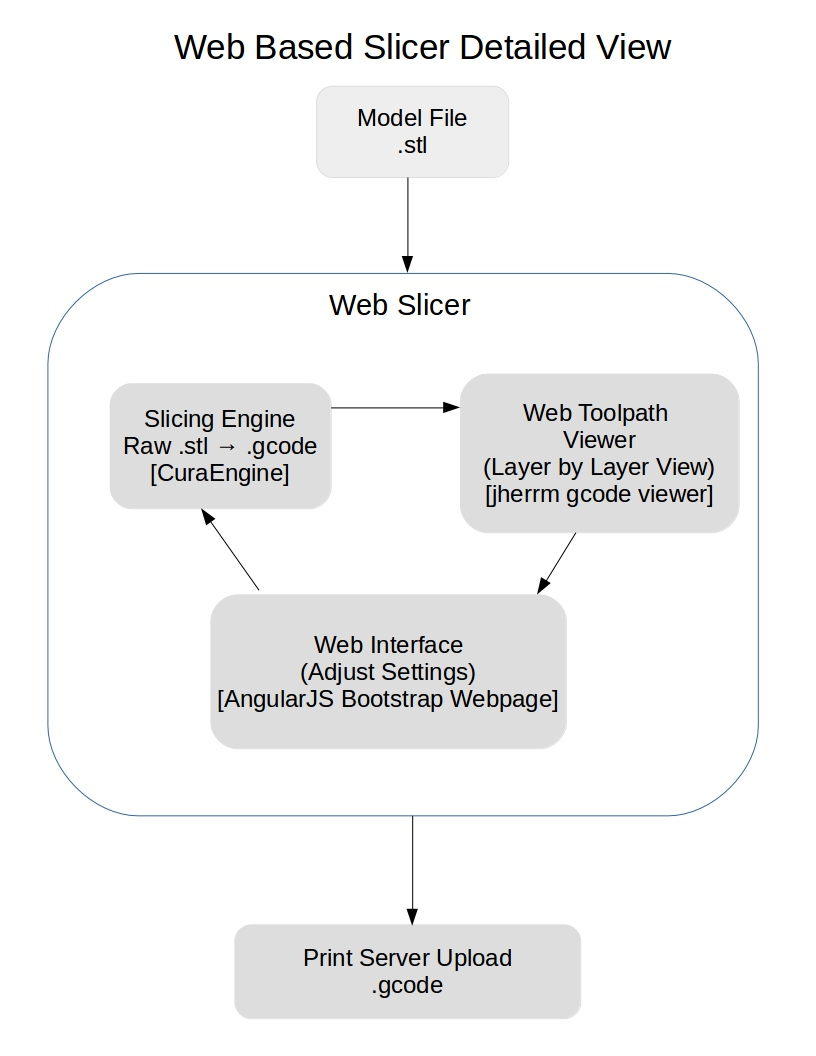
\includegraphics[width=\linewidth]{slicer-detailed-view}
  \caption{High level view of how WebSlicer functions and how users will interact with it}
  \label{fig:slicer-detailed-view}
\end{figure}

\section{Working Procedure}
\paragraph{}
% this needs way more info
As shown in Figure \ref{fig:slicer-detailed-view}, the application will have 3 major components that all need to work together in a cycle until the user decides that the output is what they desire.

\subsection{Web Interface}
\paragraph{}
The web interface includes a set of forms for collecting the user's settings for their printer and the settings as they relate to printing the model itself.
This interface also includes a method so the user may retain the files they have uploaded for future use.
This does not include the actual slicing engine, which must be driven and accessed independently.

\subsection{Slicing Engine}
\paragraph{}
To comprehend the slicing engine it is vital to understand what G-code is.
G-code consists of sequential machine instructions that command a 3D printer to move in a sequence of patters to build a three dimentional part \citep{gcode-2012}.
Listing \ref{lst:gcode} shows a sample of G-code that results from slicing using CuraEngine.
Comments in G-code are preceded by a semicolon and the first line denotes the type of G-code, we are only focusing on RepRap G-code in this case.
Commands in G-code follow a standard pattern of a letter, either M or G, and a number which denotes the type of command.
All subsequent items that are separated by spaces are arguments to the command.

% JSON settings example listing
\begin{lstlisting}[language=json, style=thesiscode , label={lst:gcode}, caption=A sample of G-code that results from slicing using CuraEngine.]
{
FLAVOR:RepRap
M190 S110.000000
M104 S245.000000
M109 S245.000000
G21 ;metric values
G90 ;absolute positioning
M82 ;set extruder to absolute mode
M107 ;start with the fan off
G28 X0 Y0 ;move X/Y to min endstops
G28 Z0 ;move Z to min endstops
G1 Z15.0 F9000 ;move the platform down 15mm
G92 E0 ;zero the extruded length
G1 F200 E3 ;extrude 3mm of feed stock
G92 E0 ;zero the extruded length again
G1 F9000
;Put printing message on LCD screen
M117 Printing...
;Generated with Cura_SteamEngine master
;LAYER_COUNT:158
;LAYER:0
M107
G0 F7200.000000 X99.430 Y80.760 Z0.300
G0 X102.806 Y78.243
;TYPE:SKIRT
G1 F1800.000 X103.337 Y78.033 E0.01074
G1 X103.441 Y77.996 E0.01282
G1 X103.842 Y77.875 E0.02070
G1 X104.142 Y77.800 E0.02651
}
\end{lstlisting}

\paragraph{}
The slicing engine rests at the core of this project as most of the computation time is spent preforming geometry calculations and converting them to G-code.
This process of converting from model to G-code is known as slicing.
An application which is encapsulated and preforms slicing is known as as a slicing engine.
The engine which carries out the raw geometry calculations for WebSlicer is CuraEngine which is written in C++.
Thus, this portion of the project required deploying the CuraEngine application on a remote server and creating a RESTful API to interface with it.

\subsection{Web Tool Path Viewer}
\paragraph{}
%expand this with more detail
After configuring and generating the G-code representation for a 3D model, there must be a way to visually review how the slicing engine will divide the model.
This is executed by loading the resulting G-code from the slicing engine into a web based visualizer.
The user is then able to view each of the layers and the steps involved in creating each one in detail.
As displayed in Figure \ref{fig:slicer-detailed-view}, this process of changing settings, slicing, and reviewing can occur an arbitrary number of times before the user decides they are satisfied with the result.

\section{Review and Usability Testing}
\paragraph{}
After preforming all steps of the working procedure, it was then necessary to test WebSlicer by running a small beta test. 
This beta test consisted of a small group of users with varying familiarity with 3D printing to test how simple WebSlicer is to use through a series of simple tasks.
These simple tasks ranged from uploading a file to finding and adjusting the correct setting for a printer.
